\documentclass[12pt]{article}

\usepackage{graphicx}
\usepackage{listings}
\usepackage{hyperref}
\usepackage{float}
\usepackage{enumitem}

\graphicspath{ {./images/} }

\oddsidemargin 0mm
\evensidemargin 0mm
\textwidth 160mm
\textheight 200mm

\pagestyle {plain}
\pagenumbering{arabic}

\newcounter{stepnum}

\title{CS/SE 2XC3 Lab 6 Report}
\author{
  Glotov, Oleg\\ L03, 400174037\\
  \texttt{glotovo@mcmaster.ca}
  \and
  Willson, Emma\\ L02, 400309856\\
  \texttt{willsone@mcmaster.ca}
  }
\date{\today}

\begin{document}

\maketitle

This report includes the main observations that we found in this week's lab, along with the analysis of our results.

\newpage 
\section{Building Heaps}
In this section, we discuss the three implementations of heap build and their time complexities. We assume that $n$ represents the size of the input array given to each build function.
\subsection{Bottom-up}
Knowing that sink has $O(\log{n})$ compexity, I would expect \verb+build_heap1()+ to have $O(n\log{n})$ complexity. This is because the function consists of a single loop that calls sink $n/2$ times. 
\subsection{Insert}
Knowing that insert has $O(\log{n})$ compexity, I would also expect \verb+build_heap2()+ to have $O(n\log{n})$ complexity. The function copies the contents of the heap into a temporary array, empties the heap, and then iteratively calls insert on each element of the heap. Since insert is called $n$ times, total complexity is $O(n\log{n})$.
\subsection{Top-down}
Knowing that sink has $O(\log{n})$ complexity, I would expect \verb+build_heap3()+ to run in $O(n\log{n})$. This is because the function calls the helper \verb+is_heap+ iteratively to check if the heap is a max heap yet. \verb+is_heap+ runs in $O(n)$ because it loops through the nonleaf nodes and checks if each node's children are both smaller than or equal to it. If not, the function calls sink on each nonleaf node in the heap. This takes $O(n\log{n})$ time, a combination of the complexity of sink and the size of $n$. 
\subsection{Experimental Method}
The method used to measure the performance of each build function was the same as the method used for lab 4. The “timeit” library was used to measure the runtime which was then exported into a csv file and subsequently analyzed in excel. The sample size for each build implementation were multiples of 10, increasing to a list size of a 1 000 000. For each sample size, an implementation was tested 5 times and the results averaged. For each trial, a new random list was generated. For experiment-related code, see the \verb+code.py+ for lab 4.
\subsection{Observations}
The complexities of the various implementations can be seen in the graph below.
\begin{figure}[H]
\centering
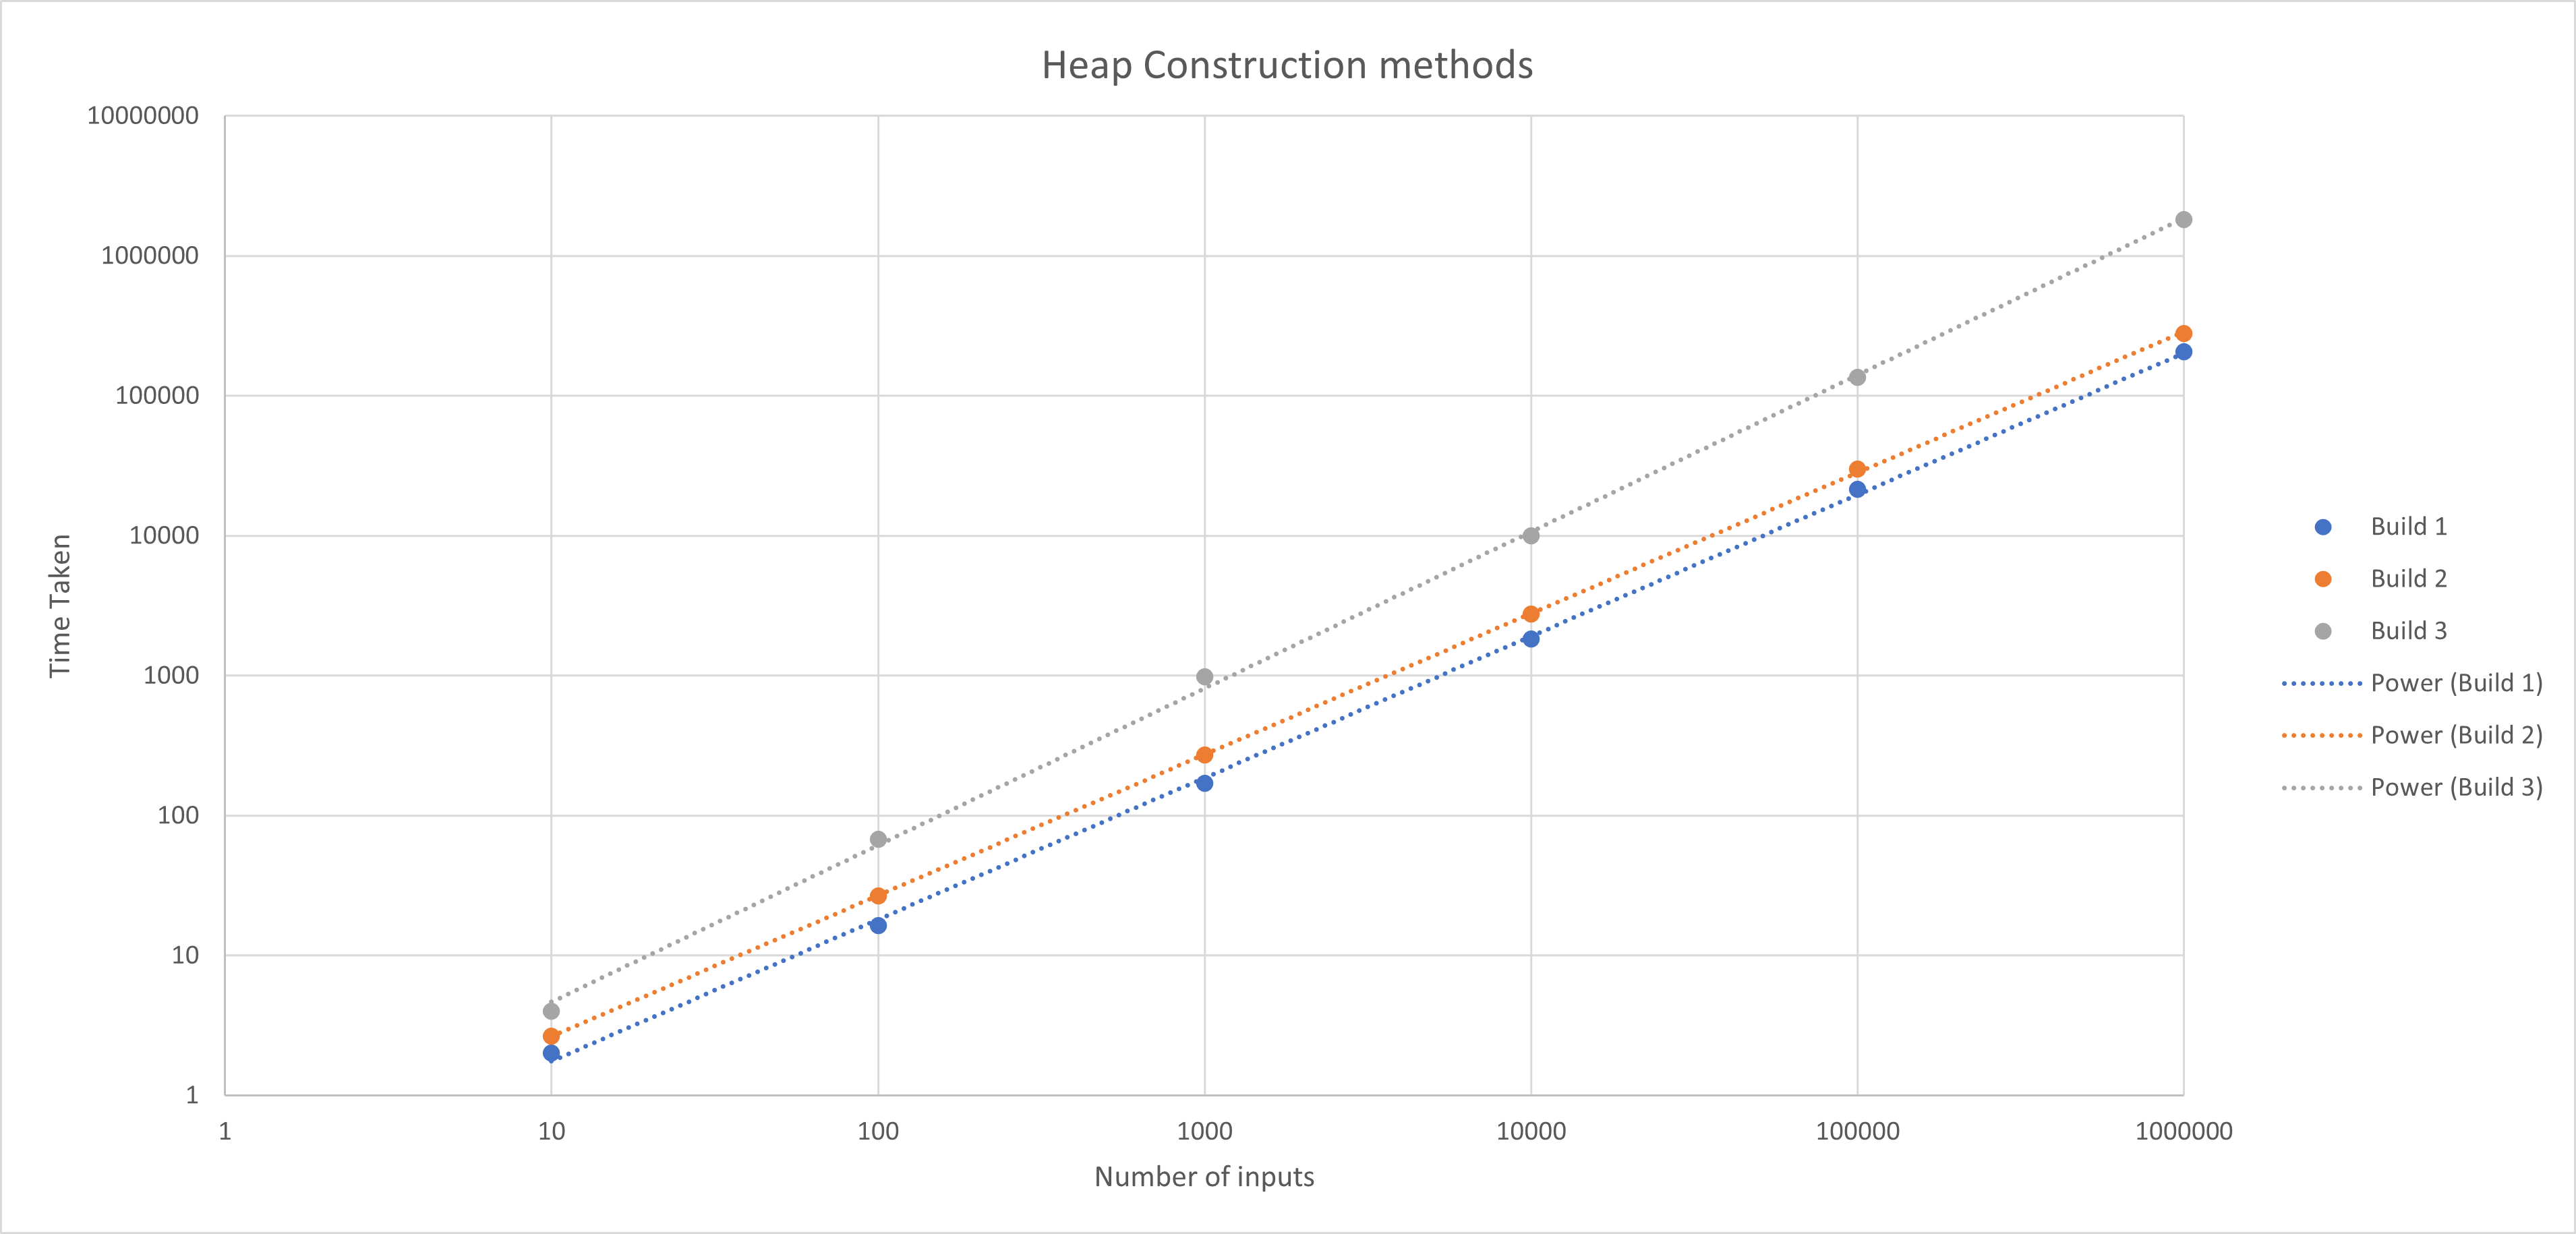
\includegraphics[width=0.9\textwidth,height=\textheight,keepaspectratio]{heap}
\caption{performance of three implementations}
\label{Figure: m1}
\end{figure}


\section{$k$-Heap}
An advantage of using a $k$-heap is that tree height is minimized. A balanced $k$-heap with $n$ elements has an insert complexity of $O(\log_k{n})$. A disadvantage of having a higher $k$ value is that it requires more compares per non-leaf node, making the overall time complexity of sinking a node, $O(k\log_k{n})$, which gets very large as $k$ increases.
I would expect our sink to have $O(k\log_k{n})$ performance because it is very similar to the sink function for binary heap except instead of doing two compares per non-leaf node, it does $k$ compares. Since 2 is a relatively small number, it can be ignored in the performance of building a binary heap. However, as $k$ gets big, I would expect this value to significantly impact performance.

\end{document}

